\documentclass[12pt]{article}
\usepackage{fullpage}
\usepackage{graphicx}
\newtheorem{definition}{Definition}
\newtheorem{question}{Question}
\newtheorem{property}{Property}
\newtheorem{proof}{\em Proof}
\newtheorem{derivation}{\em Sketch}
\newtheorem{notation}{Notation}

\newcommand{\comment}[1]{}
\newcommand{\VS}{\mbox{\it VS}}
\newcommand{\WM}{\mbox{\it WM}}
\newcommand{\PCONJ}{\mbox{\it PCONJ}}
\newcommand{\kDNF}{\mbox{\it kDNF}}
\newcommand{\PDISJ}{\mbox{\it PDISJ}}
\newcommand{\DTrt}{\mbox{\it DT}_{r2}}
\newcommand{\DTs}{\mbox{\it DT}_s}
\newcommand{\PP}{{\rm P}}
\newcommand{\EE}{{\rm E}}
\newcommand{\PX}{\PP_{\!\scriptscriptstyle\! X}}
\newcommand{\PXY}{\PP_{\!\scriptscriptstyle\! X\!Y}}
\newcommand{\PYX}{\PP_{\!\scriptscriptstyle\! Y\!|\!X}}
\newcommand{\PYx}{\PP_{\!\scriptscriptstyle\! Y\!|x}}
\newcommand{\seq}[1]{\langle{#1}\rangle}
\newcommand{\RR}{I\!\!R}
\newcommand{\NN}{I\!\!N}
\newcommand{\argmin}{\arg\!\min}
\newcommand{\argmax}{\arg\!\max}
\newcommand{\eg}{{\em e.g.},\ }
\newcommand{\Eg}{{\em E.g.},\ }
\newcommand{\ie}{{\em i.e.},\ }
\newcommand{\Ie}{{\em I.e.},\ }
\newcommand{\cf}{{\em cf.}\ }
\newcommand{\etc}{{\em etc}}
\newcommand{\aka}{{\em a.k.a.}}
\newcommand{\vardef}{\stackrel{\triangle}{=}}
\def\norm [#1]{{\| #1 \|}}
\newcommand{\sign}{\mbox{\rm sign}}
\newcommand{\err}{\mbox{\rm err}}
\newcommand{\rank}{\mbox{\rm rank}}
\newcommand{\cond}{\mbox{\rm cond}}
\newcommand{\vect}{\mbox{\rm vec}}
\newcommand{\tr}{\mbox{\rm tr}}
\newcommand{\set}[1]{{\{#1\}}}
\newcommand{\tnorm}[2]{\|{#1}\|_{#2}}
\newcommand{\normdot}{{\mbox{$\|\!\cdot\!\|$}}}

%\newcommand{\makevector}[1]{{\tilde{#1}}}
\newcommand{\makevector}[1]{{\bf #1}}
\newcommand{\fvec}{{\makevector{f}}}
\newcommand{\evec}{{\makevector{e}}}
\newcommand{\bvec}{{\makevector{b}}}
\newcommand{\rvec}{{\makevector{r}}}
\newcommand{\dvec}{{\makevector{d}}}
\newcommand{\xvec}{{\makevector{x}}}
\newcommand{\qvec}{{\makevector{q}}}
\newcommand{\yvec}{{\makevector{y}}}
\newcommand{\mvec}{{\makevector{m}}}
\newcommand{\vvec}{{\makevector{v}}}
\newcommand{\zvec}{{\makevector{z}}}
\newcommand{\avec}{{\makevector{a}}}
\newcommand{\wvec}{{\makevector{w}}}
\newcommand{\cvec}{{\makevector{c}}}
\newcommand{\Xvec}{{\makevector{X}}}
\newcommand{\Fvec}{{\makevector{F}}}
\newcommand{\Avec}{{\makevector{A}}}
\newcommand{\Bvec}{{\makevector{B}}}
\newcommand{\Hvec}{{\makevector{H}}}
\newcommand{\Lvec}{{\makevector{L}}}
\newcommand{\Mvec}{{\makevector{M}}}
\newcommand{\Nvec}{{\makevector{N}}}
\newcommand{\Vvec}{{\makevector{V}}}
\newcommand{\Uvec}{{\makevector{U}}}
\newcommand{\Ivec}{{\makevector{I}}}
\newcommand{\Ovec}{{\makevector{O}}}
\newcommand{\smallxvec}{{\scriptsize\mathbf x}}
\newcommand{\alphavec}{\mbox{\boldmath $\alpha$}}
\newcommand{\betavec}{\mbox{\boldmath $\beta$}}
\newcommand{\muvec}{\mbox{\boldmath $\mu$}}
\newcommand{\phivec}{{\mbox{\boldmath $\phi$}}}
\newcommand{\lambdavec}{\mbox{\boldmath $\lambda$}}
\newcommand{\Lambdavec}{\mbox{\boldmath $\Lambda$}}
\newcommand{\Sigmavec}{\mbox{\boldmath $\Sigma$}}
\newcommand{\yy}{{\tt y}}
\newcommand{\uu}{{\tt u}}
\newcommand{\zerovec}{{\makevector{0}}}
\newcommand{\smallzerovec}{{\scriptsize\bf 0}}
\newcommand{\smallonevec}{{\scriptsize\bf 1}}
\newcommand{\onevec}{{\makevector{1}}}
\newcommand{\smallbetavec}{\mbox{\scriptsize\boldmath $\beta$}}
\newcommand{\smallmuvec}{\mbox{\scriptsize\boldmath $\mu$}}


\begin{document}

\noindent
{\Large\bf AUCSC 460 -- Artificial Intelligence}

\vspace*{1\baselineskip}

\noindent
{\large\bf Assignment 5: Classification}

\vspace*{1\baselineskip}

\noindent
Winter 2016\\
Department of Science\\
University of Alberta, Augustana Faculty\\
{\bf Instructor}: Anna Koop, HB 1-31, akoop@ualberta.ca

\vspace*{1.75\baselineskip}
\hrule

\begin{tabbing}
{\bf Instructor}:\ \ \=\kill
\>{\bf Due}:\'{\em Friday, Apr 8 at 23:55:00 local time}
\\
\>{\bf Worth}:\' 25\% of final grade \\
\>(5 questions worth 5\% each)
\end{tabbing}

\hrule

\vspace*{1.25\baselineskip}

\noindent
{\bf Note}:
Through eclass, submit a single file called models.py defining the specified functions.

\subsubsection*{Handwritten digit recognition}

In this assignment you will implement handwritten digit recognizers using simple probability models.
We will be using a simplified version of the MNIST data we saw before. The data files can be checked out of the class repository. The file {\tt digits.csv} contains the templates for each digit (the first row is the template label). The {\tt digit.X.csv} files contain 1100 samples of {\tt X} digit.
% noise     0.0025    0.0125    0.0350    0.9000    0.0350    0.0125    0.0025
% htrans    0.5625    0.2500    0.1875
% vtrans    0.2500    0.5625    0.1875

\bigskip

\noindent
{\em Background}:
In this assignment digit images will be represented by $8\times8$
arrays of greyscale numbers, where
1 = black, 2 = dark grey, 3 = light grey, and 4 = white.
For example, the following matrix represents the corresponding image.

\bigskip

\hspace*{1.5cm}
\raisebox{2.5cm}{$\left[\begin{array}{cccccccc}
     1 &     1 &     1 &     2 &     3 &     4 &     4 &     4 \\
     1 &     1 &     2 &     3 &     4 &     2 &     2 &     2 \\
     1 &     1 &     3 &     4 &     2 &     1 &     1 &     1 \\
     1 &     2 &     4 &     4 &     4 &     4 &     2 &     1 \\
     1 &     1 &     2 &     2 &     2 &     2 &     4 &     2 \\
     2 &     1 &     1 &     1 &     2 &     3 &     4 &     2 \\
     4 &     3 &     2 &     2 &     3 &     4 &     2 &     1 \\
     2 &     4 &     4 &     4 &     4 &     2 &     1 &     1
\end{array}\right]$}

\begin{figure}[bt]
\centering
\caption{Handwritten 5}
\label{fig:five}
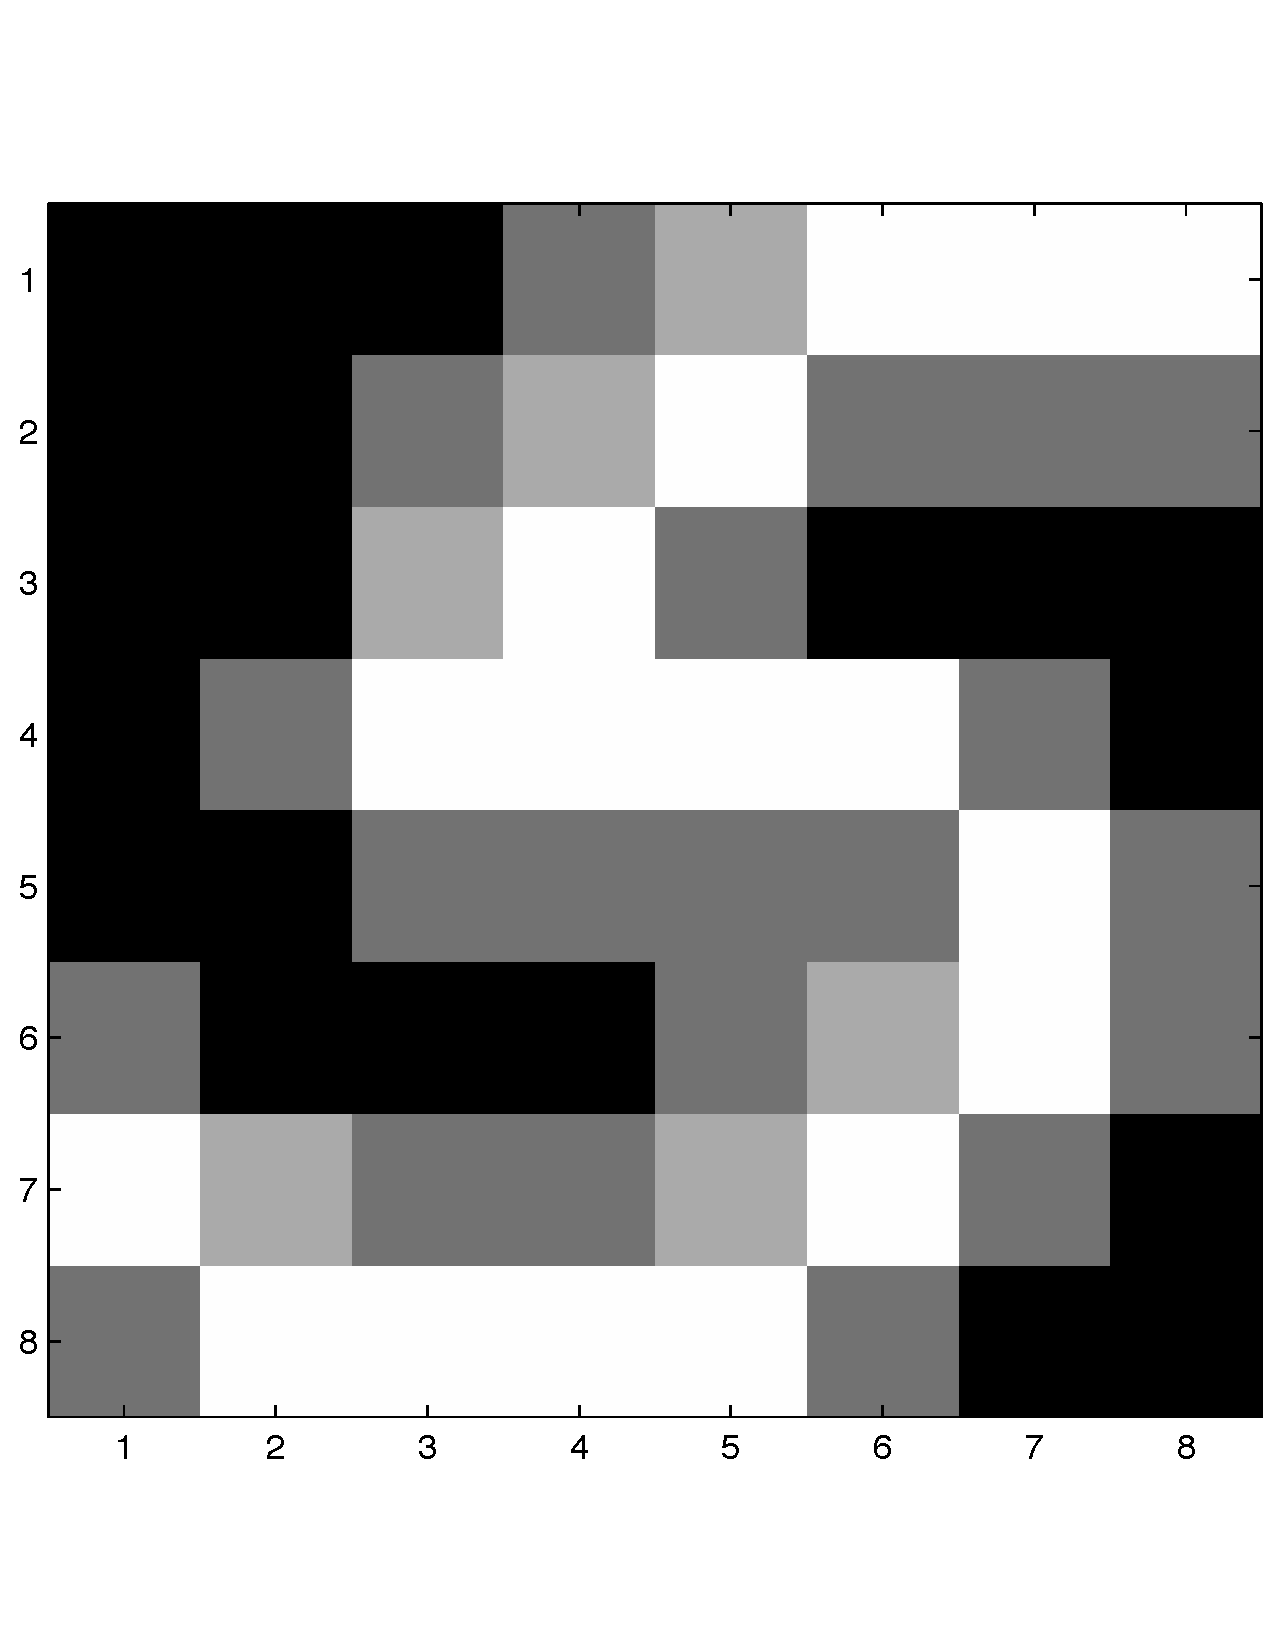
\includegraphics[width=2in]{images/five.pdf}
\end{figure}
%\quad
%\epsfxsize=2in\epsfbox{five.eps}

The assignment is split up into two main parts: in the first part
you will implement a generator and recognizer for two different
probability models (where the second model extends the previous).
In the second part you will implement a classifier of your choice.

%\vspace*{1\baselineskip}
\newpage

\hrule

\section{Simplest Probabilistic Model}
\label{sec:prob1}
%%%%%%%%%%%%%%%%%%%%%%%%%%%%%%%%%%%%%%%%%%%%%%%%%%%%%%%%%%%%%%%%%%%%%%%%%%%%

\setlength{\unitlength}{0.00083300in}%
%
\begingroup\makeatletter\ifx\SetFigFont\undefined%
\gdef\SetFigFont#1#2#3#4#5{%
  \reset@font\fontsize{#1}{#2pt}%
  \fontfamily{#3}\fontseries{#4}\fontshape{#5}%
  \selectfont}%
\fi\endgroup%
\hspace*{1.5in}
\begin{picture}(2100,2150)(901,-2261)
\thicklines
\put(2401,-286){\circle{336}}
\put(2401,-886){\circle{336}}
\put(2401,-1486){\circle{336}}
\put(2401,-2086){\circle{336}}
\put(1726,-1486){\circle{336}}
\put(2401,-436){\vector( 0,-1){300}}
\put(2401,-1036){\vector( 0,-1){300}}
\put(2401,-1636){\vector( 0,-1){300}}
\put(1876,-1486){\vector( 1, 0){375}}
\put(3001,-961){\makebox(0,0)[lb]{\smash{\SetFigFont{12}{14.4}{\rmdefault}{\mddefault}{\updefault}digit template value}}}
\put(3001,-1561){\makebox(0,0)[lb]{\smash{\SetFigFont{12}{14.4}{\rmdefault}{\mddefault}{\updefault}raw pixel value}}}
\put(3001,-2161){\makebox(0,0)[lb]{\smash{\SetFigFont{12}{14.4}{\rmdefault}{\mddefault}{\updefault}observed pixel value}}}
\put(901,-1561){\makebox(0,0)[lb]{\smash{\SetFigFont{12}{14.4}{\rmdefault}{\mddefault}{\updefault}noise}}}
\put(2251,-361){\makebox(0,0)[lb]{\smash{\SetFigFont{12}{14.4}{\rmdefault}{\mddefault}{\updefault}{\footnotesize digit}}}}
%\put(2326,-961){\makebox(0,0)[lb]{\smash{\SetFigFont{12}{14.4}{\rmdefault}{\mddefault}{\updefault}$d_{ij}$}}}
\put(2300,-961){\makebox(0,0)[lb]{\smash{\SetFigFont{12}{14.4}{\rmdefault}{\mddefault}{\updefault}$d_{ij}$}}}
%\put(1651,-1561){\makebox(0,0)[lb]{\smash{\SetFigFont{12}{14.4}{\rmdefault}{\mddefault}{\updefault}$n_{ij}$}}}
\put(1625,-1561){\makebox(0,0)[lb]{\smash{\SetFigFont{12}{14.4}{\rmdefault}{\mddefault}{\updefault}$n_{ij}$}}}
%\put(2326,-1561){\makebox(0,0)[lb]{\smash{\SetFigFont{12}{14.4}{\rmdefault}{\mddefault}{\updefault}$r_{ij}$}}}
\put(2300,-1561){\makebox(0,0)[lb]{\smash{\SetFigFont{12}{14.4}{\rmdefault}{\mddefault}{\updefault}$r_{ij}$}}}
%\put(2326,-2161){\makebox(0,0)[lb]{\smash{\SetFigFont{12}{14.4}{\rmdefault}{\mddefault}{\updefault}$o_{ij}$}}}
\put(2300,-2161){\makebox(0,0)[lb]{\smash{\SetFigFont{12}{14.4}{\rmdefault}{\mddefault}{\updefault}$o_{ij}$}}}
\end{picture}


\noindent
Pick a digit $n$ uniformly at random from among 0,1,...,9.
and retrieve its corresponding image template $D$ (a 64-element vector corresponding to an $8\times8$ array).
Given the digit template, each image pixel $o_{ij}$ is generated independently 
by first picking a random noise value $n_{ij}\in\{-3,-2,-1,0,1,2,3\}$
(according to the distribution defined in {\tt noise}),
adding the noise to the corresponding digit template pixel $d_{ij}$
to obtain the raw pixel value, $r_{ij}=d_{ij}+n_{ij}$,
and then thresholding the raw value to obtain the observed image pixel:
\[
o_{ij} \;\;=\;\;\left\{\begin{array}{cll}
r_{ij} & \mbox{ if } & 1\leq r_{ij}\leq4\\
1 & \mbox{ if } & r_{ij} < 1\\
4 & \mbox{ if } & r_{ij} > 4
\end{array}\right.
\]
The {\tt noise} vector gives the probability of obtaining each noise value:
{\tt noise(1)}$=\PP(n_{ij}\!=\!-3)$,
{\tt noise(2)}$=\PP(n_{ij}\!=\!-2)$,
...,
{\tt noise(7)}$=\PP(n_{ij}\!=\!3)$.

%%%%%%%%%%%%
\subsection{Generation \rm(Model 1---5\%)}

Write a  function {\tt simplegen(digits, noise)} that, given a dictionary of template {\tt digits} and probability vector for weighting the noise values,
 returns a random image of a digit generated by the model outlined above.

A simple noise vector to try is $ [0.0025,    0.0125,    0.0350,    0.9000,    0.0350,    0.0125,    0.0025]$ (note that this is heavily weighted toward 0, which does not alter the pixel value).


\subsection{Recognition \rm(Model 1---5\%)}

Given an observed image $O$, we wish to compute the most likely
digit given the image.  This amounts to computing the most likely
digit image template $D$ given $O$
(since digits and their image templates are in a one-to-one correspondence).
Thus, we wish to find

\begin{eqnarray*}
D^* & = & \arg\max_D \; \PP(D|O)
\\
& = & \arg\max_D \; \PP(DO)
\\
& = & \arg\max_D \; \sum_N \PP(DNO)
\\
& = & \arg\max_D \; \sum_N \PP(D) \PP(N) \PP(O|DN)
\\
& = & \arg\max_D \; \PP(D) \sum_{n_{11}=-3}^3\cdots\sum_{n_{88}=-3}^3 \left[\prod_{i=1}^8\prod_{j=1}^8\PP(n_{ij})\right]\left[\prod_{i=1}^8\prod_{j=1}^8\PP(o_{ij}|d_{ij},n_{ij})\right]
\\
& = & \arg\max_D \; \PP(D) \prod_{i=1}^8\prod_{j=1}^8 \sum_{n_{ij}=-3}^3 \PP(n_{ij})\PP(o_{ij}|d_{ij},n_{ij})
\end{eqnarray*}
where
\[
\PP(o_{ij}|d_{ij},n_{ij}) \;\;=\;\;\left\{
\begin{array}{ll}
1 & \begin{array}[t]{l}\mbox{ if } d_{ij}+n_{ij}=o_{ij}\\
                    \mbox{ or } o_{ij} = 1 \mbox{ and } d_{ij}+n_{ij}<1\\
                    \mbox{ or } o_{ij} = 4 \mbox{ and } d_{ij}+n_{ij}>4\\
\rule{0em}{1ex}
    \end{array}
\\
0 & \mbox{ otherwise }
\end{array}
\right.
\]
and $P(D)$ is uniform.
For each digit image template, $D^{(1)},...,D^{(9)},D^{(0)}$,
we can then compute the conditional probability of $D^{(d)}$ given
$O$ by $\PP(D^{(d)}|O)=\PP(D^{(d)}O)/\sum_{d=1,...9,0}\PP(D^{(d)}O)$.

\bigskip

%%%%%%%%%%%%
Write a function {\tt simplerec(obs, digits, noise)}, where {\tt obs} is
a 64-element vector representing the $8\times8$ image of an observed digit, 
and {\tt digits} and {\tt noise} are as before. Your recognition function 
returns the array {\tt probs}, a $1\times10$ array of the conditional
probabilities of each digit given {\tt obs}. Note that {\tt argmax(probs)} tells you the most-likely class.

The classification and conditional probabilities are to be calculated
using the procedures outlined above.
(Note that the conditional probabilities may be near zero or one.)


\vspace*{1\baselineskip}

%%%%%%%%%%%%%%%%%%%%%%%%%%%%%%%%%%%%%%%%%%%%%%%%%%%%%%%%%%%%%%%%%%%%%%%%%%%%
%\newpage
\hrule

\section{Multi-step Probabilistic Model}

The second probability model extends the first by adding a possible 
transformation to the digit templates before generating the final image.
We will consider a small set of simple 
horizontal and vertical shear transformations.
In particular, horizontal shear transformations
will slide the top part of the image template to the left
and the bottom part to the right.
For example, a horizontal shear value of $h=2$ 
will shift the template as follows:

%\setlength{\unitlength}{3947sp}%
\setlength{\unitlength}{3730sp}%
%
\begingroup\makeatletter\ifx\SetFigFont\undefined%
\gdef\SetFigFont#1#2#3#4#5{%
  \reset@font\fontsize{#1}{#2pt}%
  \fontfamily{#3}\fontseries{#4}\fontshape{#5}%
  \selectfont}%
\fi\endgroup%
\begin{picture}(3624,2424)(589,-2773)
\thinlines
\put(1201,-361){\line( 0,-1){2400}}
\put(1201,-2761){\line( 1, 0){2400}}
\put(3601,-2761){\line( 0, 1){2400}}
\put(3601,-361){\line(-1, 0){2400}}
\put(1201,-361){\line(-1, 0){600}}
\put(601,-361){\line( 0,-1){600}}
\put(601,-961){\line( 1, 0){2400}}
\put(3001,-961){\line( 0, 1){600}}
\put(901,-961){\line( 0,-1){600}}
\put(901,-1561){\line( 1, 0){2400}}
\put(3301,-1561){\line( 0, 1){600}}
\put(3301,-961){\line(-1, 0){300}}
\put(3301,-1561){\line( 1, 0){300}}
\put(1201,-1861){\line( 1, 0){2700}}
\put(3901,-1861){\line( 0,-1){600}}
\put(3901,-2461){\line(-1, 0){2400}}
\put(1501,-2461){\line( 0, 1){600}}
\put(1801,-2461){\line( 0,-1){300}}
\put(3601,-2761){\line( 1, 0){600}}
\put(4201,-2761){\line( 0, 1){300}}
\put(4201,-2461){\line(-1, 0){300}}
\put(601,-661){\line( 1, 0){2400}}
\put(901,-1261){\line( 1, 0){2400}}
\put(1501,-2161){\line( 1, 0){2400}}
\end{picture}

%\quad
%\raisebox{-1.1ex}{\epsfxsize=2in\epsfbox{shearfive.eps}}

\noindent
Similarly, a vertical shear transformation will
slide the left part of the image
in an opposite direction to the right part.
For example, a vertical shear value of $v=-1$
will shift the template as follows:

\bigskip

\hspace*{2.2em}
%\setlength{\unitlength}{3947sp}%
\setlength{\unitlength}{1900sp}
%
\begingroup\makeatletter\ifx\SetFigFont\undefined%
\gdef\SetFigFont#1#2#3#4#5{%
  \reset@font\fontsize{#1}{#2pt}%
  \fontfamily{#3}\fontseries{#4}\fontshape{#5}%
  \selectfont}%
\fi\endgroup%
\begin{picture}(4824,6024)(1189,-5773)
\thinlines
\put(1201,-361){\line( 1, 0){4800}}
\put(6001,-361){\line( 0,-1){4800}}
\put(6001,-5161){\line(-1, 0){4800}}
\put(1201,-5161){\line( 0, 1){4800}}
\put(4801,-5161){\line( 0, 1){4800}}
\put(3601,-361){\line( 0,-1){4800}}
\put(4201,-361){\line( 0,-1){4800}}
\put(3001,-361){\line( 0,-1){5400}}
\put(3001,-5761){\line(-1, 0){1800}}
\put(1201,-5761){\line( 0, 1){600}}
\put(1201,-961){\line( 1, 0){1800}}
\put(2401,-961){\line( 0,-1){4800}}
\put(1801,-961){\line( 0,-1){4800}}
\put(4801,-4561){\line( 1, 0){1200}}
\put(4801,-361){\line( 0, 1){600}}
\put(4801,239){\line( 1, 0){1200}}
\put(6001,239){\line( 0,-1){600}}
\put(5401,239){\line( 0,-1){4800}}
\end{picture}

\hspace*{1.49cm}
%\raisebox{2.3ex}{\epsfxsize=2in\epsfbox{shearvfive.eps}}

Generation from this model is similar to before,
except that we introduce an intermediate transformation
step which takes into account both the horizontal and
vertical shears.

\begin{center}
%\setlength{\unitlength}{3947sp}%
\setlength{\unitlength}{0.00083300in}%
%
\begingroup\makeatletter\ifx\SetFigFont\undefined%
\gdef\SetFigFont#1#2#3#4#5{%
  \reset@font\fontsize{#1}{#2pt}%
  \fontfamily{#3}\fontseries{#4}\fontshape{#5}%
  \selectfont}%
\fi\endgroup%
\begin{picture}(1702,2750)(1550,-2861)
\thinlines
\put(2401,-2686){\circle{336}}
\put(1726,-2086){\circle{336}}
\put(3076,-1486){\circle{336}}
\put(1876,-2086){\vector( 1, 0){375}}
\put(2401,-2236){\vector( 0,-1){300}}
\put(2926,-1486){\vector(-1, 0){375}}
\put(2326,-961){\makebox(0,0)[lb]{\smash{\SetFigFont{12}{14.4}{\rmdefault}{\mddefault}{\updefault}{$D$}%
}}}
\put(2326,-1561){\makebox(0,0)[lb]{\smash{\SetFigFont{12}{14.4}{\rmdefault}{\mddefault}{\updefault}{$W$}%
}}}
\put(2326,-2161){\makebox(0,0)[lb]{\smash{\SetFigFont{12}{14.4}{\rmdefault}{\mddefault}{\updefault}{$R$}%
}}}
\put(2326,-2761){\makebox(0,0)[lb]{\smash{\SetFigFont{12}{14.4}{\rmdefault}{\mddefault}{\updefault}{$O$}%
}}}
\put(1651,-2161){\makebox(0,0)[lb]{\smash{\SetFigFont{12}{14.4}{\rmdefault}{\mddefault}{\updefault}{$N$}%
}}}
\put(1651,-1561){\makebox(0,0)[lb]{\smash{\SetFigFont{12}{14.4}{\rmdefault}{\mddefault}{\updefault}{$h$}%
}}}
\put(3001,-1561){\makebox(0,0)[lb]{\smash{\SetFigFont{12}{14.4}{\rmdefault}{\mddefault}{\updefault}{$v$}%
}}}
\put(2401,-286){\circle{336}}
\put(2401,-886){\circle{336}}
\put(2401,-1486){\circle{336}}
\put(2401,-2086){\circle{336}}
\put(1726,-1486){\circle{336}}
\put(2401,-436){\vector( 0,-1){300}}
\put(2401,-1036){\vector( 0,-1){300}}
\put(2401,-1636){\vector( 0,-1){300}}
\put(1876,-1486){\vector( 1, 0){375}}
\put(2251,-361){\makebox(0,0)[lb]{\smash{\SetFigFont{12}{14.4}{\rmdefault}{\mddefault}{\updefault}digit}}}
\end{picture}

\end{center}

To generate an image, 
pick a digit $n$ uniformly at random 
and retrieve its corresponding image template $D$.
Then independently pick a random horizontal shear number $h\in\{0,1,2\}$
(according to the distribution defined in {\tt htrans}),
and
a random vertical shear number $v\in\{-1,0,1\}$
(according to the distribution defined in {\tt vtrans}).
Then, given $D$, $h$ and $v$, a warped template $W$ is created according to

\[
w_{ij} \;\;=\;\;\left\{
\begin{array}{ll}
d_{\;t(j,i,v)\;t(i,j,h)}
& \mbox{ if both $1\leq t(j,i,v)\leq 8$ and $1\leq t(i,j,h)\leq 8$}
\\[2ex]
1 & \mbox{ otherwise}
\end{array}
\right.
\]
where
%
\begin{eqnarray*}
t(j,i,v) & = & i+round(v(5-j)/4)
\\
t(i,j,h) & = & j+round(h(5-i)/4)
\end{eqnarray*}
%
Note that the
{\tt htrans} vector gives the probability of obtaining each 
horizontal shear value:
{\tt htrans(1)}$=\PP(h\!=\!0)$,
{\tt htrans(2)}$=\PP(h\!=\!1)$,
{\tt htrans(3)}$=\PP(h\!=\!2)$;
and
the {\tt vtrans} vector gives the probability of obtaining each 
vertical shear value:
{\tt vtrans(1)}$=\PP(v\!=\!-1)$,
{\tt vtrans(2)}$=\PP(v\!=\!0)$,
{\tt vtrans(3)}$=\PP(v\!=\!1)$.

Finally, given the warped template, each image pixel $o_{ij}$ is generated 
independently as before by
first picking a random noise value $n_{ij}$ and adding it to
$w_{ij}$ to obtain a raw pixel value $r_{ij}=w_{ij}+n_{ij}$,
and then thresholding between 1 and 4 to obtain the final observed value.
%The overall generative model is summarized in the following diagram.
 
%%%%%%%%%%%%
\subsection{Generation \rm(Model 2---5\%)}
 Write a function {\tt transformgen(digits, noise, htrans, vtrans)} that 
returns a random image of a digit generated by the model outlined above.

Example {\tt htrans} $[0.5625,    0.2500,   0.1875]$ and {\tt vtrans} $[0.2500,    0.5625,    0.1875]$.



\vspace*{1\baselineskip}

%%%%%%%%%%%%%%%%%%%%%%%%%%%%%%%%%%%%%%%%%%%%%%%%%%%%%%%%%%%%%%%%%%%%%%%%%%%%
%\newpage
\hrule

\subsection{Recognition \rm(Model 2---5\%)}

\begin{eqnarray*}
D^*
& = & \arg\max_D \; \PP(DO)
\\
& = & \arg\max_D \; \sum_h\sum_v\sum_N \PP(D)\PP(h)\PP(v)\PP(N)\PP(O|D,h,v,N)
\\
& = & \arg\max_D \; \PP(D)\sum_h\PP(h)\sum_v\PP(v)\sum_{n_{11}}\cdots\sum_{n_{88}} 
\left[\prod_i\prod_j\PP(n_{ij})\right]
\left[\prod_i\prod_j \PP(o_{ij}|d_{\;t(j,i,v)\;t(i,j,h)\;},n_{ij}) \right]
\\
& = & \arg\max_D \; \PP(D)\sum_h\PP(h)\sum_v\PP(v)
\prod_i\prod_j \sum_{n_{ij}} \PP(n_{ij})\PP(o_{ij}|d_{\;t(j,i,v)\;t(i,j,h)\;},n_{ij})
\end{eqnarray*}

where %$t(i,j,s)=j+\mbox{round}(s(5-i)/4)$
%and 
$\PP(o_{ij}|d_{\;t(j,i,v)\;t(i,j,h)\;},n_{ij})$ is determined as before.


%%%%%%%%%%%%
\bigskip

Write a function {\tt transformrec(obs, digits, noise, htrans, vtrans} that returns an $1\times10$ array of the conditional
probabilities of each digit given {\tt obs}.
The classification and conditional probabilities are to be calculated
using the procedures outlined above.


\vspace*{1\baselineskip}


\bigskip
\hrule

%%%%%%%%%%%%
\section{Classification \rm(Your Choice---5\%)}
Write a {\tt Classifier} class that defines two methods: {\tt train} and {\tt test}. You may use the classification method of your choice. The training function {\tt train(X, y)} takes an $t*n$ matrix of input data, with the corresponding $t$ labels. The testing function takes an $m*n$ matrix of input data and returns a vector of the corresponding $m$ labels.

Document the assumptions your classifier makes about the input data and labels. Test it on the {\tt digit} data files as well as on your own generated models. 

Note that the 1100 images in each {\tt digit.X.csv} forms a very large set
and it would probably take too long to test your model on every image.
Instead, you can (repeatedly) test the model on 25 randomly chosen
images for each digit.
(The instructor will apply a similar test to verify that your model is indeed
an improvement.)

\end{document}